\chapter{Risk Assessment and Mitigation}
\section{Introduction}
Throughout the project we will face a number of potential risks however we will do our best to mitigate them.
When analysing the risks we will focus on two factors, likelihood and severity.

A risk can either have a high, medium, or low chance of becoming a reality.
If a problem is not likely to occur when running a project three times or more we deem it to have a low likelihood.
If it is likely to occur once during the project or when running a project twice we deem it medium likelihood.
Finally, if it is likely to occur multiple times during the project, we will deem it as high likelihood.

A risk can also either be high, medium, or low in severity.
A high severity risk could result in months of lost progress up to having to totally start over.
A medium severity risk could result in the loss of between one week and a few weeks of progress.
Finally a low severity risk would only result in a maximum of a few days of lost progress.

To combine these two factors into something meaningful we will use a risk matrix (Figure~\ref{fig:risktable}).
This will allow us to find a balance and identify the risks that will pose major problems.

\begin{figure}[h]
	\begin{centering}
		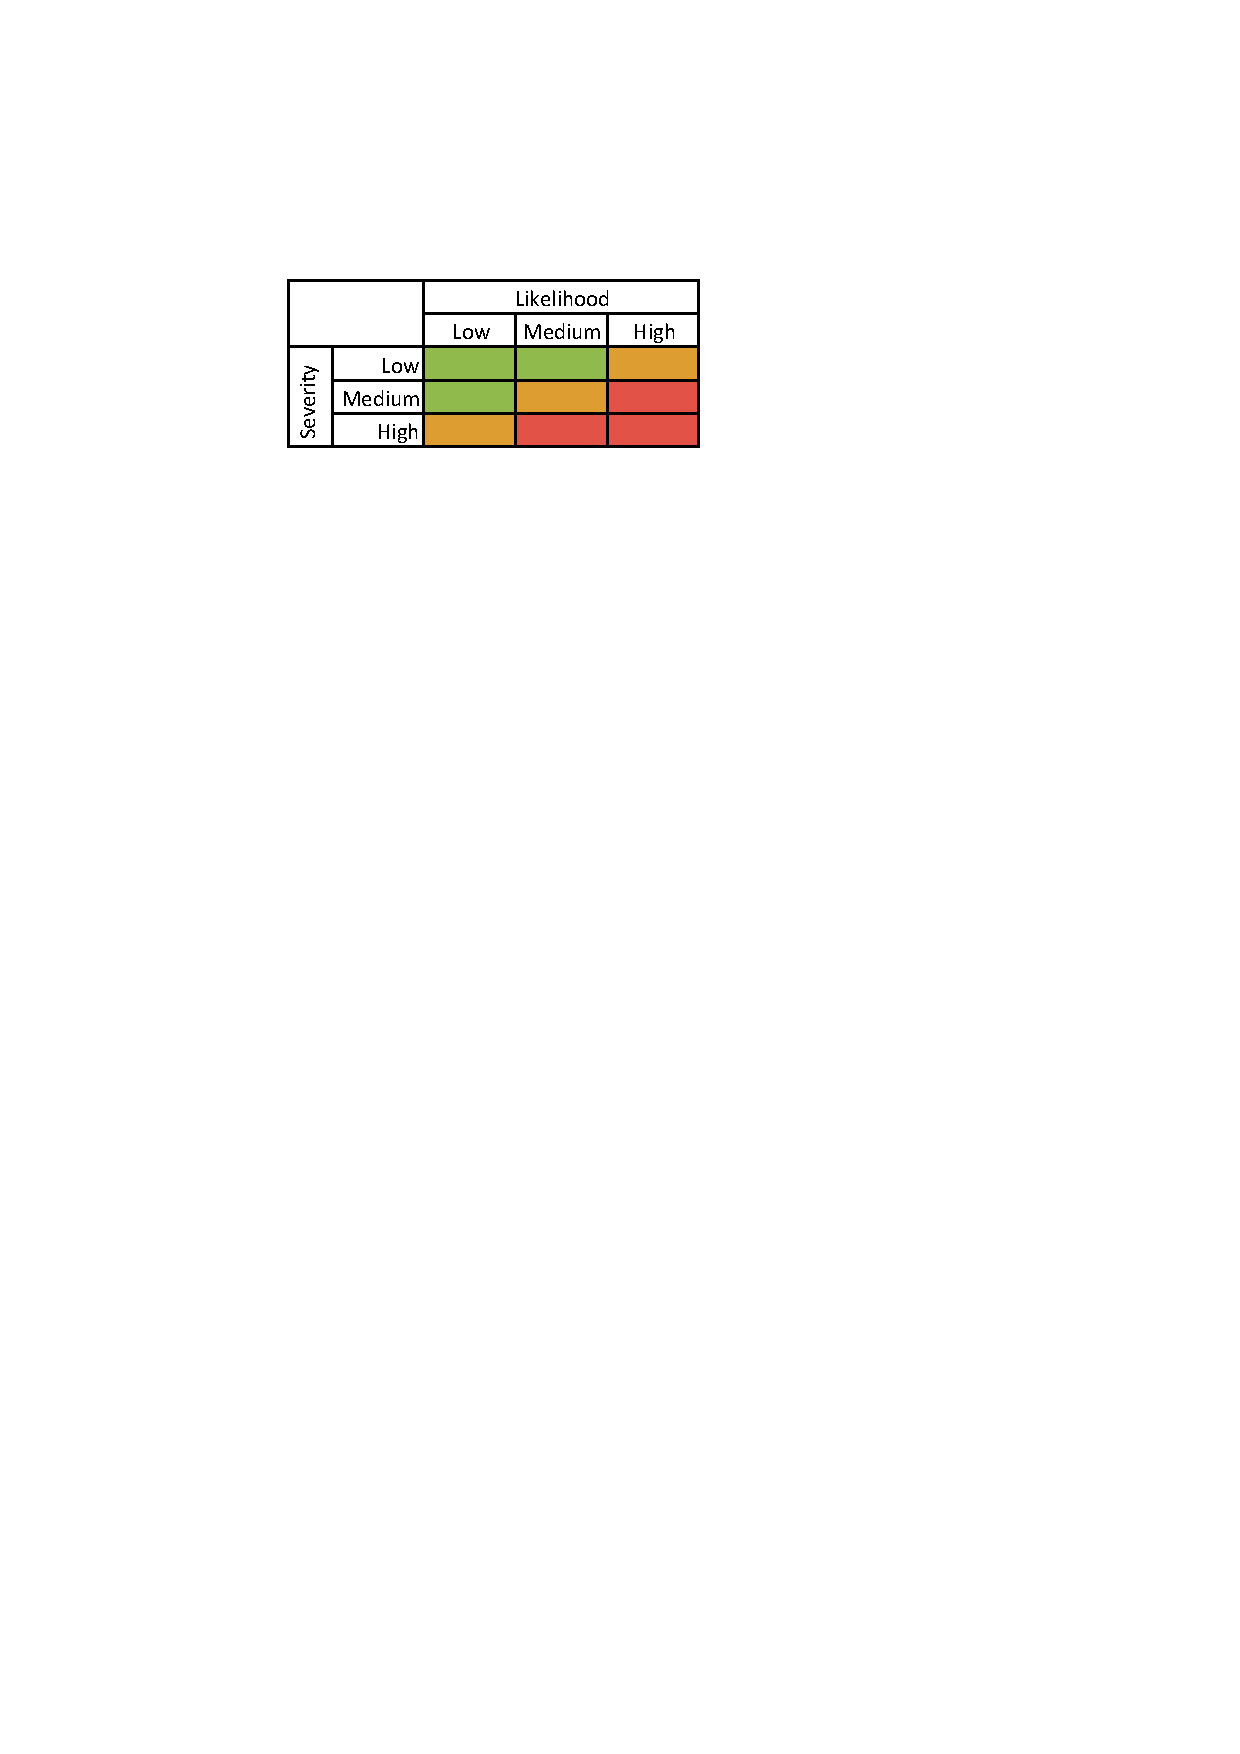
\includegraphics{risktable.pdf}
		\caption{Table showing how likelihood and severity of a risk combine to show overall impact of the risk}
		\label{fig:risktable}
	\end{centering}
\end{figure}

Green cells in the matrix are considered to be overall low risk, this is because they are not particularly likely to happen and if they do they will not have be severe enough to majorly impact the project.
Orange cells signify an overall medium risk.
They are either likely to happen but low severity, very unlikely to happen but would have a very severe impact or somewhere between.
Overall high severity risks, red cells, are the most important to mitigate.
They have a reasonably high chance of happening and could result in the loss of weeks or months of work.

It is important to categorise risks once they have been identified so that we can prioritise mitigation, it is imperative that overall high risks cannot happen and in the case that they do we must be able to cope with them and have protocols in place to lessen the impact.

We will be presenting the risks in a risk register with columns identifying, analysing and showing the mitigations for the risk.
This will give us an accessible and easily modifiable document which we will be able to use throughout the project when considering or attempting to mitigate risks.

\newpage

\begin{landscape}
\section{Risk Assessment}
\begin{longtable}{|l|p{5cm}|l|l|l|p{4cm}|p{5cm}|}
	\hline
	\textbf{Category} & \textbf{Name} & \textbf{Severity} & \textbf{Likelihood} & \textbf{Overall} & \textbf{Mitigation} & \textbf{Contingency} \\ \hline \hline
	\endhead
	Staff & Team member leaves & High & Low & Medium & & \\ \hline
	Staff & Staff sick or unable to attend meetings. & Medium & High & High & Let other members of the team know as soon as possible & Other staff takes over their work temporarily. \\ \hline
	Staff & Don’t have the skill required to complete the task. & Low & Medium & Low & Research the skills needed. Ask other team members if they know how to help. & Read books and the internet about required skills. \\ \hline
	Staff & Staff don’t listen others opinion& Low & Low & Low & More communication, consult Richard/Fiona if the problem continues. & Stay together and work out the root reason, then resolve it. \\ \hline
	
	Staff/Requirements & Staff failed to complete the task before deadline. & High & Low & Medium & More rapid sprint to ensure everyone is on track. & Cut our optional features and complete the compulsory requirements first. \\ \hline
	
	Requirements & Change of requirements & Low & High & Medium & Keep in touch, build and show to the client & Update the requirement document and update the product. \\ \hline
	Requirements & Responsible of telling the customer that requirements were impossible and offer alternative options. & Low & Low & Low & Negotiate with the customer before updating the requirements. & Explain to the customer what has to be changed. \\ \hline
	Requirements & Cannot meet the requirement & High & Low & Medium & Design realistic requirements before start coding. & Modify the requirements so it can be met. \\ \hline
	
	Tech & Data lost - e.g. hard drive failure. & Medium & Low & Low & Backup data regularly to cloud or different devices. & Restore most recent backed up data. \\ \hline
	Tech & IT facility failure & Low & Low & Low & Routine maintenance to devices. & Use campus computer to continue development. \\ \hline
	Tech & Security threats & High & Low & Medium &  Install antivirus software and enable firewall. & Seek IT support for help and continue working. \\ \hline
	Tech & Software bug that causes data loss. & High & Medium & High & Backup data before executing dangerous commands. & Reset to the previous commit using git. \\ \hline
	
	Tools & Tools not available & Low & Medium & Low & Research background information about alternatives before proceeding. & Switch to an alternative tool, request help from IT support or create one if enough time before deadline. \\ \hline
	Tools & Unfamiliar with the toolset. & Low & Medium & Low & Learn how to use the tool. & Ask IT support or other teammates for help. \\ \hline
	Tools & Tools does not fit into the project after start off. & Low & Medium & Low & Do extensive research and comparison before integrating to the workflow. & Find alternative and re-evaluate options. \\ \hline
	
	Estimation & Estimates that there will not be enough time to finish the whole project. & High & Medium & High & Allocate and plan the time efficiently. & Plan and spend more time for the project. \\ \hline
	
	Customer & Customer changes the requirements. & Low & High & Medium & Keep in touch and understand the necessary changes as soon as possible. & Examine new requirements and update them accordingly. \\ \hline
	Customer & Customer doesn't allow or understand why we have to change the requirements. & Medium & Medium & Medium & Keep in touch with the customer & Sit next with the customer and talk through the reason why. \\ \hline
	
	Test & Bugs discovered & Medium & High & High & Understand the code and have comments around them. & Fix bugs. \\ \hline
	Test & Something wrong but cannot find the errors. & Medium & Medium & Medium & Put comment around the code to describe, and do tests. & Debug the problem using a debugger and seek for help. \\ \hline
	
\end{longtable}
\end{landscape}